\begin{figure*}[ht!]
\centering
%-------------------------------------------------
% First row: two line plots side by side
%-------------------------------------------------
\hspace{-1.6cm}
\begin{subfigure}[b]{0.45\textwidth}
    \begin{tikzpicture}
\begin{axis}[
    width=1.1\linewidth,
    height=0.7\linewidth,
    title={\emph{High-Speed} Models on ImageNet-1K at $224^2$ px},
    title style={yshift=-5pt},
    xlabel={Throughput (K images/s)},
    xlabel shift=-5pt,
    ylabel={Top-1 Acc. ($\%$)},
    ylabel shift=-5pt,
    xmin=5.75, xmax=45,
    ymin=59, ymax=83.5,
    grid=major,
    line width=1pt
]
% \shade[
%     right color=yellow!60,
%     left color=white,
%     middle color=white,
%     samples=100,
%     opacity=0.2
% ] (rel axis cs:0,1) -- (rel axis cs:1,1) -- (rel axis cs:1,0) -- cycle;

% \shade[
%     top color=yellow!60,
%     bottom color=white,
%     middle color=white,
%     samples=100,
%     opacity=0.2
% ] (rel axis cs:0,1) -- (rel axis cs:1,1) -- (rel axis cs:1,0) -- cycle;

% \node[anchor=south west] at (rel axis cs:0.82,0.85) {\small optimal};
% ------------------------------------------------------
% 1) EFFICIENTVIT (ICCV 2023)
% ------------------------------------------------------
\draw[\efficientColor, line width=1.5pt, style=dashed]
  (axis cs:25.328, 66.3) coordinate (B1)
  -- (axis cs:9.553, 76.9) coordinate (B2)
  node[midway, above, sloped, xshift=75pt, yshift=-6pt] {\small EfficientViT};

\EfficientMarker[1.0]{(B1)}
\EfficientMarker[1.0]{(B2)}

% ------------------------------------------------------
% 2) SHVIT (CVPR 2024)
% ------------------------------------------------------
\draw[\shvitColor, line width=1.5pt, style=dashed]
  (axis cs:40.913, 67.9) coordinate (S1)
  -- (axis cs:33.828, 71.0) coordinate (S2)
    node[midway, above, sloped] {\small SHViT};

\draw[\shvitColor, line width=1.5pt, style=dashed]
  (S2)
  -- (axis cs:23.081, 74.3) coordinate (S3);

\ShvitMarker[1.0]{(S1)}
\ShvitMarker[1.0]{(S2)}
\ShvitMarker[1.0]{(S3)}

% ------------------------------------------------------
% 3) MOBILENETV4 (ECCV 2024)
% ------------------------------------------------------
\draw[\mobileColor, line width=1.5pt, style=dashed]
  (axis cs:33.136, 65.6) coordinate (M1)
  -- (axis cs:10.403, 74.9)  coordinate (M2)
    node[midway, above, sloped, xshift=25pt] {\small MobileNetV4};
    
\draw[\mobileColor, line width=1.5pt, style=dashed]
  (M2)
  -- (axis cs:8.121, 78.1)  coordinate (M3);

\MobileMarker[2.0]{(M1)}
\MobileMarker[2.0]{(M2)}
\MobileMarker[2.0]{(M3)}

% ------------------------------------------------------
% 4) VIT+REGISTERS (ICLR 2024)
% ------------------------------------------------------
\draw[\registerColor, line width=1.5pt]
  (axis cs:26.042, 61.0) coordinate (R1)
  -- (axis cs:16.711, 74.5)  coordinate (R2)
      node[midway, below, sloped, xshift=13pt] {\small ViT+Registers};

\draw[\registerColor, line width=1.5pt]
  (R2)
  -- (axis cs:6.865, 81.9)  coordinate (R3);
% \draw[\registerColor, line width=1.5pt]
%   (axis cs:26.042, 61.0) coordinate (R1)
%   -- (axis cs:16.711, 74.5)  coordinate (R2)
%   -- (axis cs:6.865, 81.9)  coordinate (R3);

% \node[color=\registerColor, anchor=east, xshift=-2pt] at (R1) {\small ViT+Registers};

\RegisterMarker[1.2]{(R1)}
\RegisterMarker[1.2]{(R2)}
\RegisterMarker[1.2]{(R3)}

% ------------------------------------------------------
% 5) VIT+JUMBO (ours)
% ------------------------------------------------------
\draw[\jumboColor, line width=1.5pt]
  (axis cs:43.137,70.5) coordinate (J0)
  -- (axis cs:31.924,74.5) coordinate (J1)
  -- (axis cs:19.938,77.7) coordinate (J2)
      node[midway, above, sloped, yshift=1pt] {\small ViT+Jumbo (ours)};
      
\draw[\jumboColor, line width=1.5pt]
  (J2)
  -- (axis cs:7.802,81.8) coordinate (J3);

\JumboMarker[0.5]{(J0)}
\JumboMarker[0.5]{(J1)}
\JumboMarker[0.5]{(J2)}
\JumboMarker[0.5]{(J3)}

\end{axis}
\end{tikzpicture}

    \phantomcaption
    \label{fig:sub:1k224}
\end{subfigure}
\hspace{0.5cm}
\begin{subfigure}[b]{0.45\textwidth}
    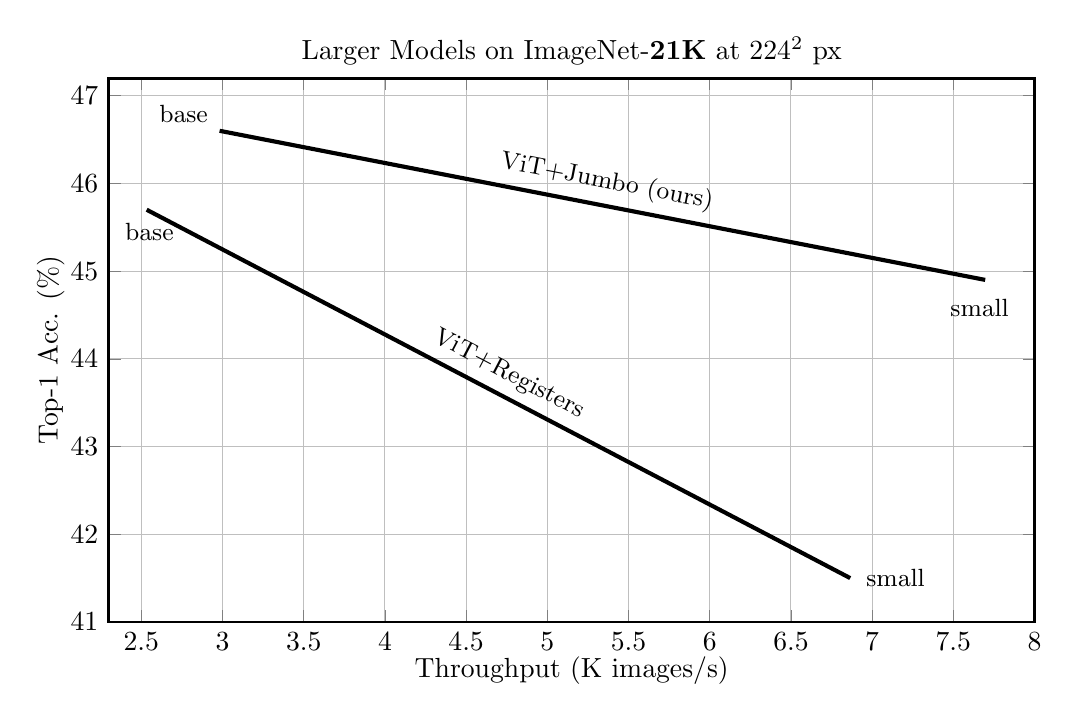
\begin{tikzpicture}
\begin{axis}[
    width=1.1\linewidth,
    height=0.7\linewidth,
    title={Larger Models on ImageNet-\textbf{21K} at $224^2$ px},
    title style={yshift=-5pt},
    xlabel={Throughput (K images/s)},
    xlabel shift=-5pt,
    ylabel={Top-1 Acc. ($\%$)},
    ylabel shift=-5pt,
    xmin=2.3, xmax=8.0,
    ymin=41., ymax=47.2,
    grid=major,
    line width=1pt
]
    % \shade[
    %     right color=yellow!60,
    %     left color=white,
    %     middle color=white,
    %     samples=100,
    %     opacity=0.2
    % ] (rel axis cs:0,1) -- (rel axis cs:1,1) -- (rel axis cs:1,0) -- cycle;
    
    % \shade[
    %     top color=yellow!60,
    %     bottom color=white,
    %     middle color=white,
    %     samples=100,
    %     opacity=0.2
    % ] (rel axis cs:0,1) -- (rel axis cs:1,1) -- (rel axis cs:1,0) -- cycle;
    
    % \node[anchor=south west] at (rel axis cs:0.82,0.85) {\small optimal};

    % --- Registers line ---
    \draw[\registerColor, line width=1.5pt]
      (axis cs:6.865,41.5) coordinate (B1)
      -- (axis cs:2.533,45.7) coordinate (B2)
      node[midway, above, sloped] {\small ViT+Registers};

    % Place Registers markers at coordinates (with full scale, here 1.0)
    \RegisterMarker[1.2]{(B1)}
    \node[right, \registerColor, xshift=2pt, yshift=0pt] at (B1) {\small small};

    \RegisterMarker[1.2]{(B2)}
    \node[below, \registerColor, xshift=1pt, yshift=-1pt] at (B2) {\small base};

    % --- Jumbo line ---
    \draw[\jumboColor, line width=1.5pt]
      (axis cs:7.696,44.9) coordinate (R1)
      -- (axis cs:2.982,46.6) coordinate (R2)
      node[midway, above, sloped] {\small ViT+Jumbo (ours)};

    \JumboMarker[0.5]{(R1)}
    \node[below, \jumboColor, xshift=-2pt, yshift=-3pt] at (R1) {\small small};

    \JumboMarker[0.5]{(R2)}
    \node[above, \jumboColor, xshift=-13pt, yshift=-1pt] at (R2) {\small base};

\end{axis}
\end{tikzpicture}
    \phantomcaption
    \label{fig:sub:21k}
\end{subfigure}

\vspace{-0.5cm}

%-------------------------------------------------
% Second row: one line plot + one table side by side
%-------------------------------------------------
\hspace{-1.6cm}
\begin{subfigure}[b]{0.45\textwidth}
    \begin{tikzpicture}
\begin{axis}[
    width=1.1\linewidth,
    height=0.7\linewidth,
    title={\emph{High-Speed} Models on ImageNet-1K at $128^2$ px},
    title style={yshift=-5pt},
    xlabel={Throughput (K images/s)},
    xlabel shift=-5pt,
    ylabel={Top-1 Acc. ($\%$)},
    ylabel shift=-5pt,
    xmin=15, xmax=140,
    ymin=52, ymax=80.5,
    grid=major,
    line width=1pt
]
% \shade[
%     right color=yellow!60,
%     left color=white,
%     middle color=white,
%     samples=100,
%     opacity=0.2
% ] (rel axis cs:0,1) -- (rel axis cs:1,1) -- (rel axis cs:1,0) -- cycle;

% \shade[
%     top color=yellow!60,
%     bottom color=white,
%     middle color=white,
%     samples=100,
%     opacity=0.2
% ] (rel axis cs:0,1) -- (rel axis cs:1,1) -- (rel axis cs:1,0) -- cycle;

% \node[anchor=south west] at (rel axis cs:0.82,0.85) {\small optimal};
% ------------------------------------------------------
% 1) EFFICIENTVIT (ICCV 2023)
% ------------------------------------------------------
\draw[\efficientColor, line width=1.5pt, style=dashed]
  (axis cs:98.585, 60.8) coordinate (B1)
  -- (axis cs:38.683, 72.8) coordinate (B2)
  node[midway, above, sloped, xshift=81pt, yshift=-7pt] {\small EfficientViT};

\EfficientMarker[1.0]{(B1)}
\EfficientMarker[1.0]{(B2)}

% ------------------------------------------------------
% 2) SHVIT (CVPR 2024)
% ------------------------------------------------------
\draw[\shvitColor, line width=1.5pt, style=dashed]
  (axis cs:79.163, 63.5) coordinate (S1)
  -- (axis cs:75.060, 66.7) coordinate (S2)
  -- (axis cs:70.458, 71.2) coordinate (S3);

\ShvitMarker[1.0]{(S1)}
\ShvitMarker[1.0]{(S2)}
\ShvitMarker[1.0]{(S3)}

\node[color=\shvitColor, anchor=west, xshift=1pt, yshift=-1pt] at (S2) {\small SHViT};

% ------------------------------------------------------
% 3) MOBILENETV4 (ECCV 2024)
% ------------------------------------------------------
\draw[\mobileColor, line width=1.5pt, style=dashed]
  (axis cs:135.663, 62.1) coordinate (M1)
  -- (axis cs:54.500, 73.3)  coordinate (M2)
  node[midway, below, sloped, xshift=35pt] {\small MobileNetV4};

\draw[\mobileColor, line width=1.5pt, style=dashed]
  (M2)
  -- (axis cs:44.325, 75.2)  coordinate (M3);

\MobileMarker[2.0]{(M1)}
\MobileMarker[2.0]{(M2)}
\MobileMarker[2.0]{(M3)}

% ------------------------------------------------------
% 4) VIT+REGISTERS (ICLR 2024)
% ------------------------------------------------------
\draw[\registerColor, line width=1.5pt]
  (axis cs:105.933, 53.6) coordinate (R1)
  -- (axis cs:52.241, 68.8)  coordinate (R2)
      node[midway, below, sloped, xshift=0pt] {\small ViT+Registers};

\draw[\registerColor, line width=1.5pt]
  (R2)
  -- (axis cs:22.176, 78.2)  coordinate (R3);


\RegisterMarker[1.2]{(R1)}
\RegisterMarker[1.2]{(R2)}
\RegisterMarker[1.2]{(R3)}

% ------------------------------------------------------
% 5) VIT+JUMBO (ours)
% ------------------------------------------------------
\draw[\jumboColor, line width=1.5pt]
  (axis cs:133.285,64.0) coordinate (J0)
  -- (axis cs:101.711,68.8) coordinate (J1)
  -- (axis cs:56.516,73.0) coordinate (J2)
      node[midway, above, sloped, yshift=2pt] {\small ViT+Jumbo (ours)};
      
\draw[\jumboColor, line width=1.5pt]
  (J2)
  -- (axis cs:19.524,78.5) coordinate (J3);

\JumboMarker[0.5]{(J0)}
\JumboMarker[0.5]{(J1)}
\JumboMarker[0.5]{(J2)}
\JumboMarker[0.5]{(J3)}

\end{axis}
\end{tikzpicture}

    \phantomcaption
    \label{fig:sub:1k128}
\end{subfigure}
\hspace{0.5cm}
\begin{subfigure}[b]{0.45\textwidth}
    \begin{figure}
    \centering
    \includegraphics[width=\linewidth]{figures/MCQA_checklist.pdf}
    \vspace{-4.75ex}
    \setlength{\fboxsep}{0pt}
    \caption{\small Example unanswerable MCQ from MMLU \cite{gema2024we}, along with rubric criteria from \citet{haladyna1989taxonomy} flagged by OpenAI's o1 \cite{jaech2024openai}.}
    \label{fig:checklist}
    \vspace{-1.7ex}
\end{figure}
    \phantomcaption
    \label{fig:sub:checklist}
\end{subfigure}

\vspace{-0.8cm}
\caption{%
ViT+Jumbo outperforms SOTA compute-efficient architectures while preserving the advantages of plain ViTs.
ViT+Jumbo equals or outperforms ViT+Registers on the standard ImageNet-1K and strictly improves on the challenging ImageNet-21K dataset.
Throughput is measured on an RTX 4090 GPU using PyTorch 2.6.0, \texttt{torch.compile}, and a $512$ batch size.
}
\label{fig:two_column_figure}
\vspace{-0.2cm}

\end{figure*}
